\section{Desarrollo}

\subsection{kNN}

El algorimo kNN (k Nearest Neighbours) se basa en el análisis de un conjunto de puntos del espacio para determinar a qué clase corresponde el nuevo objeto. En este caso cada imagen estará representada como un vector donde cada elemento es un píxel distinto de la misma. El conjunto de puntos elegido serán aquellas $k$ imágenes que más cerca se encuentren de la imagen a clasificar. Lo que se hace es clasificar a la nueva imagen como la clase que mayor representantes tenga en este conjunto de puntos cercanos.

Este algoritmo puede ser sumamente costoso en cuanto al tiempo de cómputo, y si la dimensión de los puntos a clasificar es muy grande, hacer uso del mismo podría resultar impracticable. Es por esto que se implementó un método cuyo objetivo es preprocesar las imágenes para reducir la cantidad de dimensiones de las muestras, permitiendo a kNN trabajar con muestras con una cantidad de variables menor. Este método es conocido como PCA (Principal components analysis).

\subsection{PCA}

El método de análisis de componentes principales se encarga de cambiar de base el conjunto de datos de entrada para obtener una mejor representación de los datos, y además reduce la dimensión de cada elemento tanto como se desee. Al reducir la dimensión de un punto es claro que se pierde determinada información sobre el mismo, pero la particularidad de este método es que, como su nombre lo indica, se queda con las componentes más importantes, dejando de lado las que menos información aporten. De este modo, la información que se descarta es la que menor relevancia tiene, por lo que se lo considera una buena manera de reducir el espacio de la entrada.

Es importante aclarar que el método no solamente reduce la dimensión de los datos, sino que cambia la base de los mismos. Por lo que es necesario tener esto en cuenta al momento de trabajar con los mismos. Si se utiliza este método para reducir la entrada de kNN, es necesario cambiar a la misma base la imagen a clasificar, de lo contrario estarían comparándose elementos que viven en distintos espacios.

\bigskip

Procedimiento para el cambio de base:

\begin{enumerate}
\item Siendo $X$ la matriz cuyas filas contienen las imágenes, se calcula $\mu = (x_1 + ... + x_n)/n$ el promedio de las imágenes, donde $x_i$ es la $i$-ésima imagen.
\item Se crea la matriz $X_\mu$ que contiene en la $i$-ésima fila al vector $(x_i - \mu)^t$
\item Se calcula la matriz de covarianza $M = X_\mu^tX_\mu$
\item Se calculan los autovectores de $M$ mediante el método de las potencias, con deflación. Cómo cada iteración en la que calculamos el autovector de la matriz en cuestión, este está asociado al autovalor de máximo módulo, los autovectores que habremos calculado se encontrarán ordenados por relevancia. De esta manera se calculan tan solo $\alpha$ autovectores, con $1 \leq \alpha \leq n$, siendo $\alpha$ la dimensión a la que se quiere reducir las imágenes. 
\item Se contruye la matriz $V$ con los autovectores calculados previamente, dispuestos como columnas. $V$ es la matriz de cambio de base.
\item Por último, se reduce la dimensión de $X$ cambiando su base. El resultado final es $V^tX^t$ que contiene la misma cantidad de imágenes pero expresadas en otra base, y en lugar de tener dimensión $n$, cada una tiene dimensión $\alpha$.
\end{enumerate}\tabularnewline

Es interesante notar que una vez hecho el cambio de base de las imágenes, éstas representan a las imágenes pero si se trata de graficarlas se obtendrá algo muy distinto a lo que era anteriormente y no podrá visualizarse nada en concreto. Solo volviendo a la base original sería posible, pero ya se habrá perdido mucha información por lo que probablemente sea difícil encontrarlo útil.

\subsection{Data augmentation}

En los métodos implementados y algoritmos similares, la performance de estos está muy relacionada a la calidad y cantidad de datos. Por este motivo se nos ocurrió que aumentar la cantidad de datos podría ser una buena idea. Tenemos la hipótesis que al realizar un “Data Augmentation”, agregando datos que podrían llegar a ser parámetros de entrada para clasificar(en nuestro caso dígitos manuscritos) obtendremos mejores resultados.

Para conseguir nuevos datos etiquetados, decidimos modificar las imágenes levemente para que estas sigan representando el mismo dígito.

Al ser dígitos manuscritos, los trazos no son perfectos, por lo que tratamos de encontrar alguna forma de aplicar transformaciones que nos generan ciertas irregularidades para imitar este comportamiento. Inspirandonos en este paper (http://citeseerx.ist.psu.edu/viewdoc/download?doi=10.1.1.160.8494\&rep=rep1\&type=pdf)
usamos una técnica que se llama deformaciones elásticas, y las implementamos en matlab generando un desplazamiento aleatorio de cada pixel y después aplicando un filtro gausseano para suavizar este desplazamiento. \\

\begin{algorithm}[H]
\NoCaptionOfAlgo
	\KwData{	
	img, $\alpha$, $\sigma$ 
	\KwResult{La imagen manipulada}
	\caption{Deformación}
	\tcc{Generamos 2 matrices de desplazamiento aleatorias} 

	dx $\leftarrow$ rand(size(img))

	dy $\leftarrow$ rand(size(img))

	\tcc{Suavizamos con un filtro gausseano la aleatoriedad de la matriz}
	fdx $\leftarrow$ $\alpha *$ imgaussfilt(dx, $\sigma$)

	fdy $\leftarrow$ $\alpha *$ imgaussfilt(dy, $\sigma$)

	\tcc{Aplica el desplazamiento aleatorio usando la interpolacion de griddata}
	res $\leftarrow$ griddata(fdx, fdy, img)
		}
\end{algorithm}

\begin{figure}[!htb]
\minipage{0.32\textwidth}
  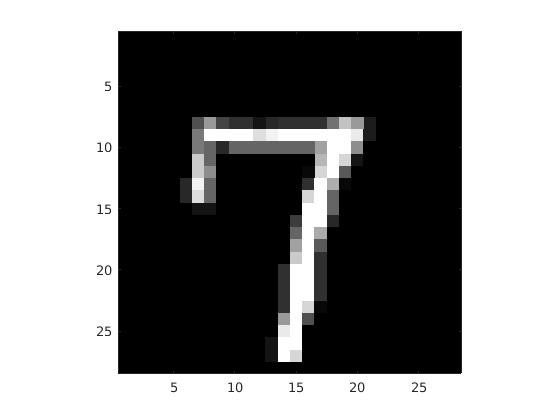
\includegraphics[width=\linewidth]{7original.jpg}
  \caption{Original}
\endminipage\hfill
\minipage{0.32\textwidth}
  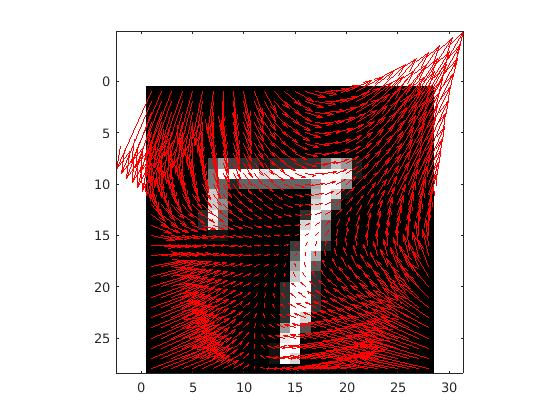
\includegraphics[width=\linewidth]{7vectpres.jpg}
  \caption{Vectores de desplazamiento}
\endminipage\hfill
\minipage{0.32\textwidth}%
  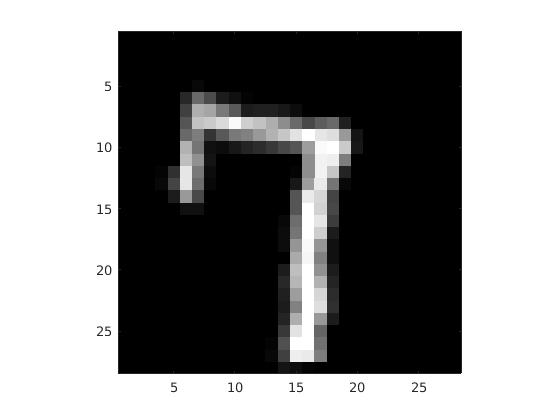
\includegraphics[width=\linewidth]{7resultado.jpg}
  \caption{Resultado}
\endminipage
\end{figure}


Como se puede observar, el dígito resultante es distinto al original pero al ojo humano sigue siendo el mismo dígito. Con este método generamos un nuevo data-set aplicando esta función a cada imagen y así ahora tenemos el doble de datos 84000 dígitos. 

Además de notar que los trazos no son perfectos, la orientación y rotación de los dígitos no es siempre la misma. Quisimos llevar al extremo aumentar los datos y aplicamos una segunda transformación a los dígitos. Para ello aplicamos una rotación aleatoria a cada dígito, usando la función de matlab para rotar imágenes imrotate, generamos un número aleatorio entre un cierto rango que le pasamos por parámetro como el ángulo. 30 grados nos pareció razonable ya que si se le aplica más hay dígitos que no se verían beneficiados.

\begin{figure}[ht] 
  \begin{minipage}[b]{0.5\linewidth}
    \centering
    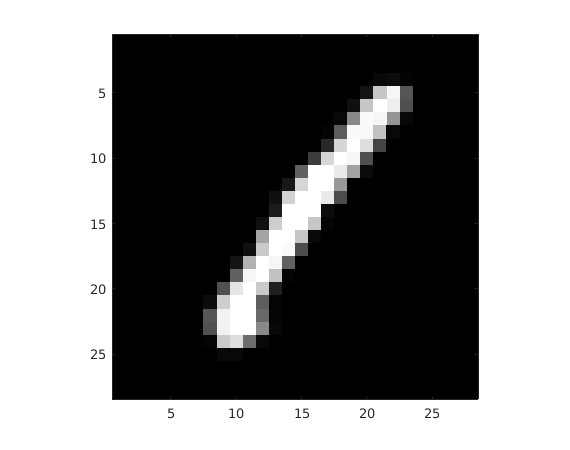
\includegraphics[width=.5\linewidth]{1_sinrotar.png} 
    \caption{Dígito Original 1} 
    \vspace{4ex}
  \end{minipage}%%
  \begin{minipage}[b]{0.5\linewidth}
    \centering
    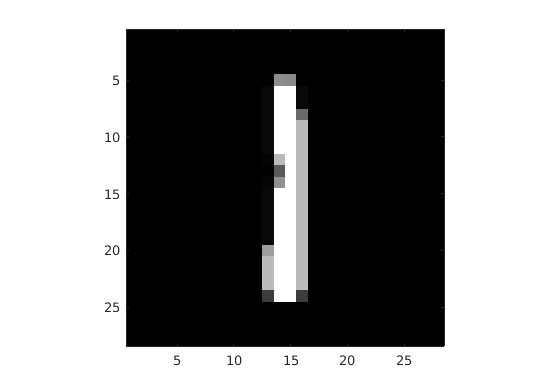
\includegraphics[width=.5\linewidth]{1_parecido.png} 
    \caption{Dígito Original 2} 
    \vspace{4ex}
  \end{minipage} 
  \begin{minipage}[b]{0.5\linewidth}
    \centering
    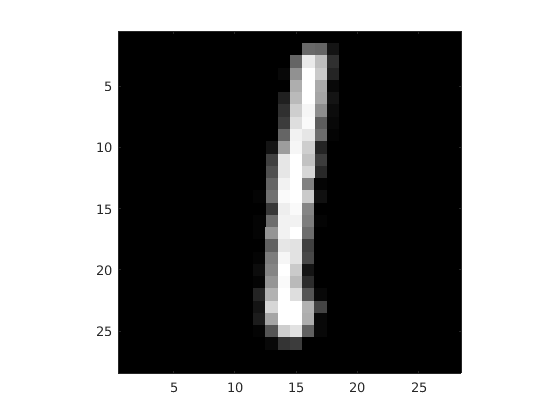
\includegraphics[width=.5\linewidth]{1_rot30.png} 
    \caption{Dígito 1 rotado $30^\circ$ sentido horario} 
    \vspace{4ex}
  \end{minipage}%% 
  \begin{minipage}[b]{0.5\linewidth}
    \centering
    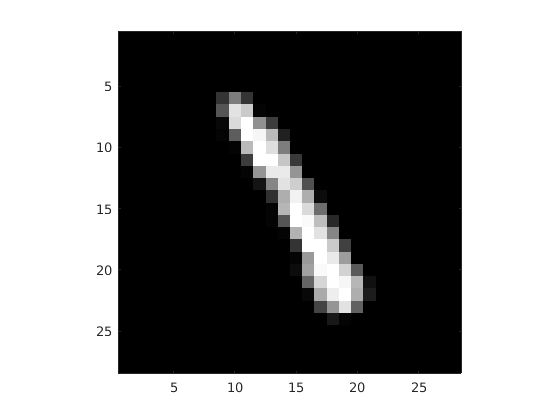
\includegraphics[width=.5\linewidth]{1_chueco.png} 
    \caption{Dígito 2 rotado $30^\circ$ sentido horario} 
    \vspace{4ex}
  \end{minipage} 
\end{figure}

En las imágenes se puede apreciar como el dígito 1 rotado es muy parecido al dígito 2, sin embargo es posible que el dígito 2 rotado pierda la esencia del dígito. Es por esta razón que optamos por usar rotaciones aleatorias.